\documentclass[]{elsarticle} %review=doublespace preprint=single 5p=2 column
\usepackage{lmodern}
\usepackage{amssymb,amsmath}
\usepackage{ifxetex,ifluatex}
\usepackage{fixltx2e} % provides \textsubscript
\ifnum 0\ifxetex 1\fi\ifluatex 1\fi=0 % if pdftex
  \usepackage[T1]{fontenc}
  \usepackage[utf8]{inputenc}
\else % if luatex or xelatex
  \ifxetex
    \usepackage{mathspec}
  \else
    \usepackage{fontspec}
  \fi
  \defaultfontfeatures{Ligatures=TeX,Scale=MatchLowercase}
\fi
% use upquote if available, for straight quotes in verbatim environments
\IfFileExists{upquote.sty}{\usepackage{upquote}}{}
% use microtype if available
\IfFileExists{microtype.sty}{%
\usepackage{microtype}
\UseMicrotypeSet[protrusion]{basicmath} % disable protrusion for tt fonts
}{}
\usepackage[margin=1in]{geometry}
\usepackage{hyperref}
\hypersetup{unicode=true,
            pdftitle={Getting Data from the Human Connectome Project (HCP)},
            pdfauthor={John Muschelli},
            pdfborder={0 0 0},
            breaklinks=true}
\urlstyle{same}  % don't use monospace font for urls
\usepackage{color}
\usepackage{fancyvrb}
\newcommand{\VerbBar}{|}
\newcommand{\VERB}{\Verb[commandchars=\\\{\}]}
\DefineVerbatimEnvironment{Highlighting}{Verbatim}{commandchars=\\\{\}}
% Add ',fontsize=\small' for more characters per line
\usepackage{framed}
\definecolor{shadecolor}{RGB}{248,248,248}
\newenvironment{Shaded}{\begin{snugshade}}{\end{snugshade}}
\newcommand{\KeywordTok}[1]{\textcolor[rgb]{0.13,0.29,0.53}{\textbf{{#1}}}}
\newcommand{\DataTypeTok}[1]{\textcolor[rgb]{0.13,0.29,0.53}{{#1}}}
\newcommand{\DecValTok}[1]{\textcolor[rgb]{0.00,0.00,0.81}{{#1}}}
\newcommand{\BaseNTok}[1]{\textcolor[rgb]{0.00,0.00,0.81}{{#1}}}
\newcommand{\FloatTok}[1]{\textcolor[rgb]{0.00,0.00,0.81}{{#1}}}
\newcommand{\ConstantTok}[1]{\textcolor[rgb]{0.00,0.00,0.00}{{#1}}}
\newcommand{\CharTok}[1]{\textcolor[rgb]{0.31,0.60,0.02}{{#1}}}
\newcommand{\SpecialCharTok}[1]{\textcolor[rgb]{0.00,0.00,0.00}{{#1}}}
\newcommand{\StringTok}[1]{\textcolor[rgb]{0.31,0.60,0.02}{{#1}}}
\newcommand{\VerbatimStringTok}[1]{\textcolor[rgb]{0.31,0.60,0.02}{{#1}}}
\newcommand{\SpecialStringTok}[1]{\textcolor[rgb]{0.31,0.60,0.02}{{#1}}}
\newcommand{\ImportTok}[1]{{#1}}
\newcommand{\CommentTok}[1]{\textcolor[rgb]{0.56,0.35,0.01}{\textit{{#1}}}}
\newcommand{\DocumentationTok}[1]{\textcolor[rgb]{0.56,0.35,0.01}{\textbf{\textit{{#1}}}}}
\newcommand{\AnnotationTok}[1]{\textcolor[rgb]{0.56,0.35,0.01}{\textbf{\textit{{#1}}}}}
\newcommand{\CommentVarTok}[1]{\textcolor[rgb]{0.56,0.35,0.01}{\textbf{\textit{{#1}}}}}
\newcommand{\OtherTok}[1]{\textcolor[rgb]{0.56,0.35,0.01}{{#1}}}
\newcommand{\FunctionTok}[1]{\textcolor[rgb]{0.00,0.00,0.00}{{#1}}}
\newcommand{\VariableTok}[1]{\textcolor[rgb]{0.00,0.00,0.00}{{#1}}}
\newcommand{\ControlFlowTok}[1]{\textcolor[rgb]{0.13,0.29,0.53}{\textbf{{#1}}}}
\newcommand{\OperatorTok}[1]{\textcolor[rgb]{0.81,0.36,0.00}{\textbf{{#1}}}}
\newcommand{\BuiltInTok}[1]{{#1}}
\newcommand{\ExtensionTok}[1]{{#1}}
\newcommand{\PreprocessorTok}[1]{\textcolor[rgb]{0.56,0.35,0.01}{\textit{{#1}}}}
\newcommand{\AttributeTok}[1]{\textcolor[rgb]{0.77,0.63,0.00}{{#1}}}
\newcommand{\RegionMarkerTok}[1]{{#1}}
\newcommand{\InformationTok}[1]{\textcolor[rgb]{0.56,0.35,0.01}{\textbf{\textit{{#1}}}}}
\newcommand{\WarningTok}[1]{\textcolor[rgb]{0.56,0.35,0.01}{\textbf{\textit{{#1}}}}}
\newcommand{\AlertTok}[1]{\textcolor[rgb]{0.94,0.16,0.16}{{#1}}}
\newcommand{\ErrorTok}[1]{\textcolor[rgb]{0.64,0.00,0.00}{\textbf{{#1}}}}
\newcommand{\NormalTok}[1]{{#1}}
\usepackage{graphicx,grffile}
\makeatletter
\def\maxwidth{\ifdim\Gin@nat@width>\linewidth\linewidth\else\Gin@nat@width\fi}
\def\maxheight{\ifdim\Gin@nat@height>\textheight\textheight\else\Gin@nat@height\fi}
\makeatother
% Scale images if necessary, so that they will not overflow the page
% margins by default, and it is still possible to overwrite the defaults
% using explicit options in \includegraphics[width, height, ...]{}
\setkeys{Gin}{width=\maxwidth,height=\maxheight,keepaspectratio}
\IfFileExists{parskip.sty}{%
\usepackage{parskip}
}{% else
\setlength{\parindent}{0pt}
\setlength{\parskip}{6pt plus 2pt minus 1pt}
}
\setlength{\emergencystretch}{3em}  % prevent overfull lines
\providecommand{\tightlist}{%
  \setlength{\itemsep}{0pt}\setlength{\parskip}{0pt}}
\setcounter{secnumdepth}{0}
% Redefines (sub)paragraphs to behave more like sections
\ifx\paragraph\undefined\else
\let\oldparagraph\paragraph
\renewcommand{\paragraph}[1]{\oldparagraph{#1}\mbox{}}
\fi
\ifx\subparagraph\undefined\else
\let\oldsubparagraph\subparagraph
\renewcommand{\subparagraph}[1]{\oldsubparagraph{#1}\mbox{}}
\fi

%%% Use protect on footnotes to avoid problems with footnotes in titles
\let\rmarkdownfootnote\footnote%
\def\footnote{\protect\rmarkdownfootnote}

%%% Change title format to be more compact
\usepackage{titling}

% Create subtitle command for use in maketitle
\newcommand{\subtitle}[1]{
  \posttitle{
    \begin{center}\large#1\end{center}
    }
}

\setlength{\droptitle}{-2em}
  \title{Getting Data from the Human Connectome Project (HCP)}
  \pretitle{\vspace{\droptitle}\centering\huge}
  \posttitle{\par}
  \author{John Muschelli}
  \preauthor{\centering\large\emph}
  \postauthor{\par}
  \predate{\centering\large\emph}
  \postdate{\par}
  \date{2016-11-18}

%%% Begin My package additions %%%%%%%%%%%%%%%%%%%
\usepackage[hyphens]{url}
\usepackage{lineno} % add
\providecommand{\tightlist}{%
  \setlength{\itemsep}{0pt}\setlength{\parskip}{0pt}}
\usepackage{graphicx}
\usepackage{booktabs} 
\usepackage{float}
\usepackage{float}
\usepackage{xcolor}
\usepackage{color}


% A modified page layout
\textwidth 6.75in
\oddsidemargin -0.15in
\evensidemargin -0.15in
\textheight 9in
\topmargin -0.5in
%%%%%%%%%%%%%%%% end my additions to header

\usepackage[T1]{fontenc}
\usepackage{lmodern}
\usepackage{amssymb,amsmath}
\usepackage{ifxetex,ifluatex}
% use upquote if available, for straight quotes in verbatim environments
\IfFileExists{upquote.sty}{\usepackage{upquote}}{}
\ifnum 0\ifxetex 1\fi\ifluatex 1\fi=0 % if pdftex
  \usepackage[utf8]{inputenc}
\else % if luatex or xelatex
  \usepackage{fontspec}
  \ifxetex
    \usepackage{xltxtra,xunicode}
  \fi
  \defaultfontfeatures{Mapping=tex-text,Scale=MatchLowercase}
  \newcommand{\euro}{€}
\fi
% use microtype if available
\IfFileExists{microtype.sty}{\usepackage{microtype}}{}
\ifxetex
  \usepackage[setpagesize=false, % page size defined by xetex
              unicode=false, % unicode breaks when used with xetex
              xetex]{hyperref}
\else
  \usepackage[unicode=true]{hyperref}
\fi
\hypersetup{breaklinks=true,
            pdfauthor={},
            pdftitle={Neuroconductor: A Framework for Reproducible Neuroimaging Analysis in R},
            colorlinks=true,
            urlcolor=blue,
            linkcolor=magenta,
            pdfborder={0 0 0}}
\urlstyle{same}  % don't use monospace font for urls
\setlength{\parindent}{0pt}
\setlength{\parskip}{6pt plus 2pt minus 1pt}
\setlength{\emergencystretch}{3em}  % prevent overfull lines
\setcounter{secnumdepth}{0}
% Pandoc toggle for numbering sections (defaults to be off)
\setcounter{secnumdepth}{0}
% Pandoc header


\newcommand{\code}[1]{\texttt{#1}}
\newcommand{\pkg}[1]{\emph{#1}}

\usepackage[nomarkers]{endfloat}
\newcommand{\fixme}[1]{{\color{red} #1}}
\begin{document}
\begin{frontmatter}

  \title{Neuroconductor: An R platform for Neuroimaging}
    \author[JHU]{John Muschelli\corref{c1}}
   \ead{jmusche1@jhu.edu} 
   \cortext[c1]{Corresponding Author}
    \author[Penn]{Jean-Philippe Fortin}
   \ead{fortin946@gmail.com} 
  
    \author[JHU]{Adrian Gherman}
   \ead{adig@jhu.edu} 
   \author[]{Brian Avants}
   \ead{stnava@gmail.com}
   
   \author[]{Brandon Whitcher}
   \ead{bwhitcher@gmail.com}   
   
    \author[JHU]{Brian S. Caffo}
   \ead{bcaffo@jhsph.edu} 
  
    \author[JHU]{Ciprian M. Crainiceanu}
   \ead{ccraini1@jhu.edu} 
  
      \address[JHU]{Johns Hopkins Bloomberg School of Public Health, Department of
Biostatistics, 615 N Wolfe St, Baltimore, MD, 21205}
    \address[Penn]{Perelman School of Medicine, University of Pennsylvania, Department of
Biostatistics and Epidemiology, 423 Guardian Drive, Philadelphia, PA
19104}
  
  \begin{abstract}
Neuroconductor \url{http://neuroconductor.org}  is an open-source platform for rapid testing and dissemination of reproducible computational imaging software. The goals of the project are to: 1) provide a centralized repository of R software dedicated to image analysis; 2) disseminate quickly software updates; 3) educate a large, diverse community of scientists using detailed tutorials and short courses; 4) ensure quality via automatic and manual quality controls; and 5) promote reproducibility of image data analysis. Based on the  programming language R (\url{https://cran.r-project.org/}), Neuroconductor starts with \fixme{24} inter-operable packages that cover multiple areas of imaging including visualization, data processing and storage, and statistical inference. Neuroconductor accepts new R package submissions, which are subject to a formal review and continuous automated testing. We provide a description of Neuroconductor's front- and back-end  and describe the user and developer experience.  
  \end{abstract}
 
 \end{frontmatter}

% Introduction
\section{Introduction}\label{introduction}

Neuroimaging software is heterogeneous, complex, and hard to use in fully reproducible analytic pipelines. These problems have been accentuated by the diversity of new imaging datasets and associated scientific problems. Indeed, many studies now collect data on thousands of subjects, at multiple visits, and using different modalities. Storing, understanding, and analyzing such data is a daunting task.  Neuroconductor will provide the software tools for using, improving and designing an open source scripted software that depends on a minimum number of software platforms and is dedicated to improving the correctness, reproducibility, and speed of neuroimage data analysis. To achieve this Neuroconductor will make no distinction between pre- and post-processing image analysis and will provide integrated data analytic approaches in R.


Neuroconductor provides data, methods, and software packages designed to support the analysis of image population studies in R, which allows integration with state-of-the-art statistical analysis software. It supports many types of imaging data including magnetic resonance imaging (MRI: structural, functional, and dynamic), computed tomography (CT), single-photon emission computed tomography, (SPECT), and magnetoencephalography (MEG). It is currently focused on human imaging, especially of the brain, but supports other biological imaging.  It can interface with mature platforms, such as Bioconductor \cite{bioc1,bioc2} and CRAN \cite{Hornik2016,r}. Neuroconductor can be used seamlessly for data fusion analyses where imaging, genomics, and other types of high-throughput data types are analyzed together with traditional measurements and health outcomes. In R these analyses can be integrated with well designed and tested analytic packages for visualization, inference, longitudinal and survival analysis, regression, network analysis, and machine learning.


\section{The user perspective}\label{section:user_perspective}
The Neuroconductor users interact with the platform via the Neuroconductor website \url{http://neuroconductor.org}. Users can install an R package, explore packages, or identify a workflow designed for their specific problem. If the workflow does not exist in Neuroconductor then users can create and submit their own workflow. 


\subsection{General description}\label{subsec:general_description}
To download a package an user would need to know the name of the package; this can be obtained from the \href{list of packages}{http://neuroconductor.org/list-current-packages} on the Neuroconductor webpage. For example, to download the packages \verb"fslr" and \verb"hcp" in R the command line instructions are 
\color{blue}
\begin{verbatim}
source("http://neuroconductor.org/neurocLite.R") 
neuro_install(c("fslr", "hcp"))
\end{verbatim}
\color{black}

Each package contains documentation as vignettes and manuals. Large areas of research covering multiple package combinations are described under Education. Some of these areas contain tutorials and Massive  Open Online Courses (MOOCs) that provide a rapid introduction of more complex concepts and workflows. Examples of such courses are Principles of fMRI  \url{https://www.coursera.org/learn/functional-mri} and Introduction to Neurohacking in R \url{https://www.coursera.org/learn/neurohacking}.  If the user does not find what they are looking for then they can develop their own tutorial and/or course that can be submitted to Neuroconductor. Furthermore, the user can turn to the Support Forum,  can attend short courses, or take free MOOCs. All package developers are users and some users become package developers.

The user starts either with their own data or downloads the data from a Neuroconductor package or using a Neuroconductor package to download it from an internet repository.  The first step is to manipulate, visualize the data, and conduct initial visual and analytic quality controls.  Most quality controls can be performed at the image or subject level, though the distribution of quality metrics in the population can be used, as well; see Mejia and al. \citep{mejia2015pca} for an example of population-level quality controls for fMRI. Once data quality has been assessed, subjects can be excluded or set aside for subsequent analyses.   

A major advantage of the R environment is that analyses can take advantage of well tested,  state-of-the-art statistical packages. For example, using demographic information,  regression, mixed effects models, or survival analysis is straightforward in R.  Results containing spatial information can be mapped back to a spatial image while results that do not can be displayed using specially designed plotting packages such as ggplot2 \citep{ggplot2}.  All of these steps can be wrapped in a series of reproducible reports using \verb"knitr" and \verb"rmarkdown" \citep{rmarkdown,knitr}. Another advantage of R is that complex processing steps and complete analyses can be wrapped into an R package. For example, the \verb"ichseg" \cite{ichseg,muschelli2016pitch} \verb"R" package is designed for intra-cranial hemorrhage segmentation and it is a wrapper for multiple functions. It uses a  single CT scan as input, processes the data using FSL \citep{fsl}, called through \texttt{fslr} \citep{fslr}, and creates a segmentation of the hemorrhagic stroke based on a pre-trained supervised machine learner. Last, packages can be deployed as Shiny applications \citep{shiny}, which are web applications built with R code and can be used by anyone with a browser.  Shiny applications can be hosted on a custom server or a Shiny server such as \url{www.shinyapps.io}. Below we provide several case studies to provide the intuition for how one could use Neuroconductor.

% Case study
\subsection{Case study: structural magnetic resonance imaging processing.} Analysis of multi-sequence structural MRI often begins with a conversion of Digital Imaging and Communications in Medicine (DICOM) files, which are essentially JPEG images with header information.  These DICOM files are converted to a Neuroimaging Informatics Technology Initiative (NIfTI), one of the most common neuroimaging formats. This process can be done in \verb"R" using the \pkg{dcm2niir} (\url{https://www.nitrc.org/projects/mricrogl/}) or \pkg{oro.dicom} \cite{dicom_nifti} packages. The resulting NIfTI files can be converted to S4 objects based on arrays using the \pkg{oro.nifti} \cite{oro.nifti} package or objects based on C++ pointers using the \pkg{ANTsR} \cite{antsr} and \pkg{RNifti} \cite{Rnifti} packages.  These packages also provide the ability to read other neuroimaging formats.

After conversion, the second step is image intensity inhomogeneity correction to ensure that each tissue has similar intensity distributions across locations in the brain (e.g. top versus bottom of the brain). Image inhomogeneities are typically caused by magnetic field inhomogeneities and can be handled by multiple methods. Neuroconductor currently contains three such methods implemented in FSL  via \pkg{fslr} \cite{zhang_segmentation_2001},  \pkg{freesurfer} \cite{sled_nonparametric_1998}, \pkg{ANTsR} \cite{sled_nonparametric_1998}, or N4 \cite{tustison_n4itk:_2010}.  

The third step is to spatially register/realign to one of the images in the sequence, usually a T1-weighted image.  This image registration can be done using \code{flirt} (\pkg{fslr}), \code{antsRegistration} (\pkg{ANTsR}), or \code{dramms} (\pkg{drammsr}).

The fourth step is brain extraction, also known as skull stripping.  This procedure is commonly done on the T1-weighted image, and can be done using \pkg{spm12r}, \pkg{fslr}, \pkg{freesurfer}, or \pkg{ANTsR}.

The fifth step is to perform an intensity normalization procedure to transform the arbitrary units in MRI into interpretable units. This is not usually thought as a standard pre-processing step, but it is crucial in many applications. For example, one could be interested in subtracting two images that were collected longitudinally to identify changes or one may want to investigate changes in voxel or ROI intensities over time.  This can be done using z-scoring with respect to a particular tissue class as implemented in WhiteStripe (\pkg{WhiteStripe}) \citep{whitestripe}, standard and robust z-scoring relative to whole brain (\pkg{neurobase}), histogram matching  (\pkg{RAVEL}), or removal of unwanted variation \citep{ravel} (\pkg{RAVEL}).  

Further subject-specific and population analyses may require registration to a population-level template. This can be done using Neurocondoctor packages within-subject registration.  Other analyses may require delineation of tissue classes of the image, which can be done using the \pkg{spm12r}, \pkg{fslr}, and \pkg{ANTsR} packages. 

% Example of a cross-package Neuroconductor workflow: preprocessing and analysis of diffusion tensor imaging data
\section{Example of a cross-package Neuroconductor workflow: preprocessing and analysis of diffusion tensor imaging data}

In this section, we discuss an example of an entire pipeline (preprocessing and statistical analysis) performed entirely with Neuroconductor.  We start with a simple question: in a population of healthy subjects, is there any difference in the white matter (WM) microstructure between males and females? Diffusion tensor imaging (DTI) is a imaging method that has been extensively used to study WM fiber structure using the differential water diffusivity of the WM in comparison to other tissues in the brain. DTI is also sensitive at capturing changes in diffusivity in the WM associated with several diseases. Fractional anisotropy (FA) and mean diffusivity (MD) are two scalar maps commonly derived from DTI images to study the diffusivity properties of the brain. 

To investigate potential gender differences between white WM fiber tracts, we use DTI images from healthy young adults from The Human Connectome Project (HCP) available at \url{db.humanconnectome.org}.  It includes a large cohort of individuals ($N > 1200$) with a vast amount of neuroimaging data ranging from structural magnetic resonance imaging (MRI), functional MRI -- both during tasks and resting-state-- and diffusion tensor imaging (DTI), \fixme{from multiple sites. JP: not sure about that. How many sites? }

% Step 1: Downloading data from the hcp package
\subsubsection{Step 1: Downloading data with the hcp package}
The first step of the pipeline is to download the minimally preprocessed DTI data \citep{hcpminimal} and structural T1w MRI images, available  for 781 subjects (436 females and 345 males) using the \texttt{hcp} \citep{hcp} package.  The \texttt{hcp} package is an R interface for downloading publicly available data from the HCP database. 

The HCP data is publicly available from Amazon Web Services (AWS). A description of how to connect to the HCP database via AWS can be found \href{https://wiki.humanconnectome.org/display/PublicData/How+To+Connect+to+Connectome+Data+via+AWS}{here}.  After accepting the data use terms, one needs to the obtain AWS credentials, which include an access key ID and a secret access key. The \texttt{hcp} package in \texttt{R} accesses the data from an Amazon Simple Storage Solution (S3) bucket using these two AWS access keys:

\color{blue}
\begin{verbatim}
library(hcp)
set_aws_api_key(access_key = "ACCESS_KEY", secret_key = "SECRET_KEY")
\end{verbatim}
\color{black}
For instance, the complete diffusion data directory for subject 100307 can be downloaded using the \verb"download_hcp_dir" function in the \texttt{hcp} package:
\color{blue}
\begin{verbatim}
result = download_hcp_dir("HCP/100307/T1w/Diffusion")
\end{verbatim}
\color{black}
and data from other subjects can be downloaded similarly. Next, after all data are downloaded, we show how to further process the DTI data using \texttt{rcamino}. 

% Step 2: Processing data with rcamino
\subsubsection{Step 2: Processing DTI data with rcamino}

We preprocess the DTI data using the Neuroconductor R package \texttt{rcamino}, an R interface for the open-source DTI software Camino \citep{camino}. The package is used to create and fit the diffusion tensor models, and to subsequently generate the fractional anisotropy (FA) and mean diffusivity (MD) scalar maps. We show below the code used for preprocessing: 

\color{blue}
\begin{verbatim}
# Extract the DTI files for the subject and name them using the nifti format
library(neurobase)
library(rcamino)
outfiles = result$output_files
names(outfiles) = neurobase::nii.stub(basename(outfiles))

# Specify the B-values and B-vectors used in the HCP database for further processing:
camino_fsl2scheme(bvecs = outfiles[["bvecs"]], bvals = outfiles[["bvals"]],
    outfile = "hcp.scheme"
)

# Convert the diffusion data from NIfTI format to Camino format:
camino_image2voxel(infile = outfiles[["data"]], outfile = "dwi.Bfloat")

# Fit the diffusion tensor imaging model:
camino_modelfit(infile = "dwi.Bfloat", outfile = "dt.Bdouble", 
    scheme = "hcp.scheme", gradadj = outfiles[["grad_dev"]],
    model = "ldt", mask = outfiles[["nodif_brain_mask"]]
)

# Produce the FA and MD maps from the fitted tensor data:
fa = camino_fa_img(infile = "dt.Bdouble", inputmodel = "dt", header = outfiles[["data"]])
md = camino_md_img(infile = "dt.Bdouble", inputmodel = "dt",header = outfiles[["data"]])
\end{verbatim}
\color{black}

We repeat this process for all subjects with available DTI data using parallel computing.

% Step 3: joint analysis
\subsubsection{Step 3: Nonlinear registration to template} 
The third step is to prepare the data for voxel-wise analysis, which requires the FA and MD maps to be spatially registered to a common template space. For each subject, we again use the \texttt{download\_hcp\_file} function to download the T1w image with extra-cranial voxels removed. We then use the diffeomorphic non-linear registration implemented in \texttt{ANTsR}, wrapped in \texttt{extrantsr}, to register FA and MD maps to the 1mm isotropic Eve template T1w image \citep{eve}, a single-subject template made available in the R package \texttt{EveTemplate}. Alternatively, one could decide to register the images to the MNI template, available in the R package \texttt{MNITemplate}.   Each registered DTI map is saved as a standard NIfTI file for further analyses. The R code is presented below.

\color{blue}
\begin{verbatim}
# Specify the path of the Eve template file:
library(EveTemplate)
eve_template = getEvePath()

# Perform non-linear registration:
t1_file = download_hcp_file("HCP/100307/T1w/T1w_acpc_dc_restore_brain.nii.gz")
reg = extrantsr::registration(filename = t1_file, 
    template.file = eve_template,	
    typeofTransform = "SyN", 
    interpolator = "Linear",
    remove.warp = FALSE
)

# Create the registered FA and MD maps:
fa_eve = ants_apply_transforms(fixed = eve_template,
    moving = fa,
    transformlist = reg$fwdtransforms
)
md_eve = ants_apply_transforms(fixed = eve_template,
    moving = md,
    transformlist = reg$fwdtransforms
)    
\end{verbatim}
\color{black}

% Step 4: statistical analysis
\subsubsection{Step 4: Statistical analysis} 

We first read the registered NIfTI files into R and create a matrix of voxels intensities with voxels as rows, and subjects as columns. We create one matrix for the FA maps, and one for the MD maps, using the  function \texttt{nifti2matrix} from the package \texttt{neurobase}. In this example, each matrix has 1,372,619 rows (number of voxels in the MNI template) and 781 columns (number of subjects in the dataset). 

There are many options in R to quantify the association of the FA and MD intensities with gender. The simplest approach is to calculate mass-univariate two-sample t-statistics (t-statistics computed at each voxel separately), which can be quickly computed using \texttt{limma}, a popular R package from the Bioconductor project \url{https://www.bioconductor.org/}. The package was originally developed for the analysis of high-throughput genomic data \citep{ritchie2015limma}, but many of the package functionalities can  applied to neuroimaging applications without any additional effort. The \texttt{limma} package also implements Empirical-Bayes (EB) methods to estimate  t-statistics based on variance shrinkage (called moderated t-statistics), which has been shown to performed well for small sample-size studies \citep{berkeley2004linear,ritchie2015limma}. The Neuroconductor package \texttt{RAVEL} contains the convenience function \texttt{getTMap}, which calculates t-statistics based on the \texttt{limma} package. 

\color{blue}
\begin{verbatim}
JP provides code here
# nifti2matrix
\end{verbatim}
\color{black}

% Step 5: Visualization of the results
\subsubsection{Step 5: Visualization of the results}


\section{The developer perspective}\label{section:dev_perspective}
To submit a package, the author/maintainer of the package will have to provide their name, a valid email address and the Github URL for the package. A short description can also be added but it is not mandatory. Once the package is submitted several initial checks will be conducted [Figure~\ref{fig:stage1}]. The checks will make sure this is a valid package with an existing DESCRIPTION file containing metadata about the package. If the initial tests are successful, an email with a random generated URL will be sent to the package maintainer to verify submission and prevent accidental/spam submissions. If the maintainer does not verify the package in a 24 hour interval, the package will be marked for deletion. 

Once the verification is complete the package will be processed [Figure~\ref{fig:stage2}]. Neuroconductor will check if this is a new package or if it is an update request for an already existing one and will either clone the package (new) or do a pull from the package GitHub (existing). The DESCRIPTION file and the .travis.yml files will be changed to reflect the Neuroconductor status for this package (\url{http://neuroconductor.org/help-package-changes} contains the complete list of changes):
\begin{enumerate}
\item original - this is a identical copy of the submitted package.
\item stable - the DESCRIPTION file and .travis.yml are modified to take into account already existing Neuroconductor stable packages.
\item development - similar to the stable, but for the existing Neuroconductor development packages.
\end{enumerate}
Next, the package will be pushed to the central Neuroconductor GitHub [\url{https://github.com/neuroconductor}] and submitted to Travis CI [\url{https://travis-ci.org/}] to be built and checked on multiple systems. The author of the package receives an automatic email indicating whether the package was built successfully and is integrated with NeuroconductoR together with a description a file containing pertinent information about the process. The package author can ask for help from the maintainers of Neuroconductor [\url{http://neuroconductor.org/contact-us}] both for compatibility issues as well as for R-specific questions. 

To write:
\begin{enumerate}
\item More sophisticated voxel-wise statistics can be easily computed within the R enviroment: glm, gee, mixed models, etc. 
\item Discuss the results, visualization and the easy use of the Eve labels to know where the differential voxels are located. 
\item Visualization of the results.
\item Should we include a plot of the results for voxel locations? Would that be a problem in terms of authorship with the HCP?
\end{enumerate}

\section{Visualization}\label{sec:visualization}

\section{Large multi-site neuroimaging data fusion}\label{sec:datafusion}
Short section about how R can be used to statistically combine large datasets using the \texttt{sva} package \citep{svapackage} that implements the SVA and ComBat methods \citep{combat}. Talk about RUV and RAVEL \citep{ravel}. 

\section{Neuroconductor infrastructure}\label{sec:backend}
The Neuroconductor project is hosted on a Red Hat Enterprise Linux Server (version 6.8 Santiago) located within the Johns Hopkins School of Public Health data center. The project architecture is based on the LAMP (\textbf{L}inux / \textbf{A}pache / \textbf{M}ySQL / \textbf{P}HP) stack, providing a flexible, fully customizable and secure end product. We are using Drupal, a CMS (\textbf{C}ontent \textbf{M}anagement \textbf{S}ystem) to provide the user interface to the Neuroconductor module. 

\begin{figure}[!ht]
  \begin{center}
    \caption{Package processing - Stage 1}
    \label{fig:stage1}
    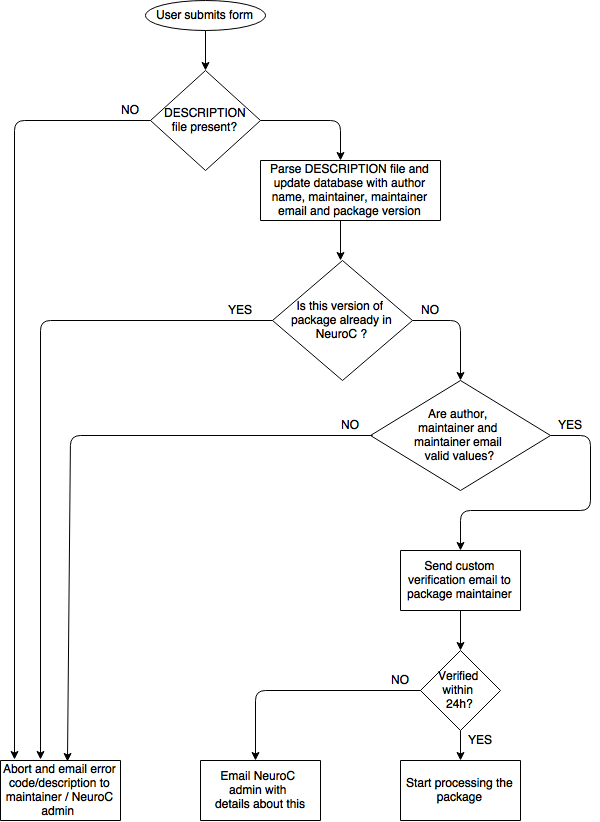
\includegraphics[height=\textheight]{flow_stage1_draft.png}\label{fig:package_lifetime_1}
  \end{center}
\end{figure}
\begin{figure}[!ht]
  \begin{center}
    \caption{Package processing - Stage 2}
    \label{fig:stage2}
    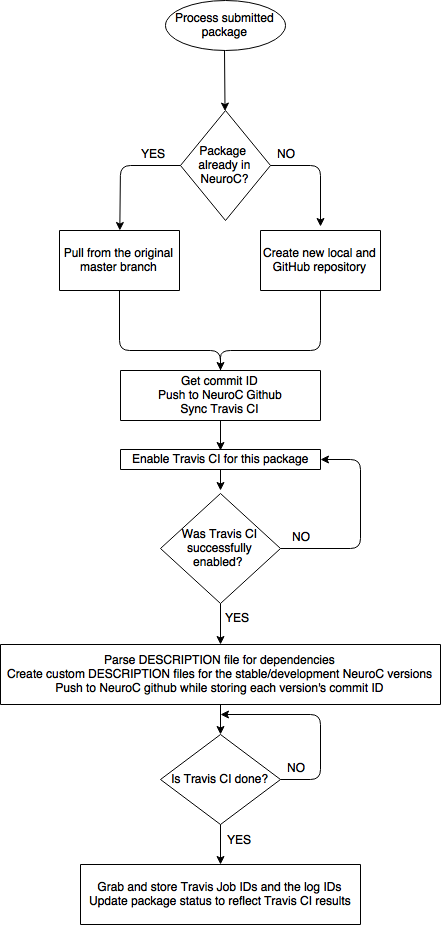
\includegraphics[height=\textheight]{flow_stage2_draft.png}\label{fig:package_lifetime_2}
  \end{center}
\end{figure}

%%%%%%%%%%%%%%%%%%%%%%%%%%%%%%%%%%%
% Table 
\begin{table}[!ht]
%\scriptsize
\centering
\caption{\textbf{Current R packages available on Neuroconductor}}\label{tab:packages}
\begin{tabular}{lll}
\hline \\[-2ex]
\textbf{Package} & \textbf{Description}   & \textbf{References} \\
\hline \\ [-1.5ex]
\multicolumn{3}{l}{\textbf{Software packages}}\\
\\ [-1.5ex]
\texttt{neurobase} & Base functions for Neuroconductor  &   \\
\texttt{oro.nifti} & Description  &  \citep{oro} \\
\texttt{oro.dicom} & Description  &  \citep{oro} \\
\texttt{oro.asl} & Description  &   \\
\texttt{oro.pet} & Description  &   \\
\texttt{ANTsR} & Advanced Normalization Tools  & \citep{ants} \\
\texttt{extrantsr} & Extensions for ANTsR  &  \\
\texttt{fslr} & R package for FSL  & \citep{fslr,fsl} \\
\texttt{freesurfer} & R package for FreeSurfer  & \citep{freesurfer} \\
\texttt{oasis} & OASIS lesion segmentation & \citep{oasis}\\
\texttt{WhiteStripe} & White Stripe intensity normalization  & \citep{whitestripe} \\
\texttt{RAVEL} & Statistical analysis of structural MRIs  & \citep{ravel} \\
\texttt{hcp} & R interface for the Human Connectome Project database &  \\
\hline \\ [-1.5ex]
\multicolumn{3}{l}{\textbf{Data packages}}\\
\\ [-1.5ex]
\texttt{kirby21.t1} &   & \citep{kirby}  \\
\texttt{kirby21.t2} &   &  \citep{kirby} \\
\texttt{kirby21.flair} &   &  \citep{kirby} \\
\texttt{kirby21.dti} &   &  \citep{kirby} \\
\texttt{kirby21.fmri} &   &  \citep{kirby} \\
\texttt{kirby21.mt} &   &  \citep{kirby} \\
\texttt{kirby21.vaso} &   &  \citep{kirby} \\
\texttt{kirby21.asl} &   &  \citep{kirby} \\
\hline \\ [-1.5ex]
\multicolumn{3}{l}{\textbf{Template packages}}\\
\\ [-1.5ex]
\texttt{MNITemplate} &   &   \\
\texttt{EveTemplate} & Eve Atlas and White Matter parcellation map  & \citep{eve}  \\
\end{tabular}
\end{table}
%%%%%%%%%%%%%%%%%%%%%%%%%%%%%%%%%%%
%%%%%%%%%%%%%%%%%%%%%%%%%%%%%%%%%%%

\subsubsection{Why R?}\label{why-r}

\begin{enumerate}
\def\labelenumi{\arabic{enumi}.}
\setcounter{enumi}{2}
\tightlist
\item
  Leverage R resources/plotting/reproducibility/package development
\item
  Leverage Bioconductor resources - they have similar problems, years of
  testing, and code
\item
  Bayesian Statistics
\end{enumerate}

\subsubsection{Third Party Software}\label{third-party-software}

FSL \citep{fsl}, AFNI \citep{afni}, FreeSurfer \citep{freesurfer}, SPM \citep{spm}


We will refer to R-Forge, OmegaHat, and CRAN as standard
repositories.



\subsection{Data Packages}\label{data-packages}

Like Bioconductor, we need data packages that allow users to test
software and examples on.

\bibliographystyle{plainnat}
\bibliography{Neuroconductor}

%\section*{References}\label{references}
%\addcontentsline{toc}{section}{References}
%
%\hypertarget{refs}{}
%\hypertarget{ref-carpux5fsecretux5f2012}{}
%Carp, Joshua. 2012. ``The Secret Lives of Experiments: Methods Reporting
%in the fMRI Literature.'' \emph{NeuroImage} 63 (1): 289--300.
%doi:\href{https://doi.org/10.1016/j.neuroimage.2012.07.004}{10.1016/j.neuroimage.2012.07.004}.
%
%\hypertarget{ref-gentleman2004bioconductor}{}
%Gentleman, Robert C, Vincent J Carey, Douglas M Bates, Ben Bolstad,
%Marcel Dettling, Sandrine Dudoit, Byron Ellis, et al. 2004.
%``Bioconductor: Open Software Development for Computational Biology and
%Bioinformatics.'' \emph{Genome Biology} 5 (10). BioMed Central: 1.

\end{document}


